\section{Parser}

Das Ziel des Parsers ist es, den Programmcode in eine Struktur zu bringen, die vom Interpreter interpretiert werden kann. Beim Lesen eines Programmcodes, wird dieser auch auf syntaktische Korrektheit überprüft. Dies geschieht mithilfe einer gegebenen Syntax in der Sprachbeschreibung.
Das Parsen wird in diesem Projekt in zwei Schritten umgesetzt. Im Unterkapitel \ref{subsection:parser} wird die Umwandlung des Programmcodes in eine Parserstruktur beschrieben. In Unterkapitel \ref{subsection:ast} wird diese dann in eine Baumstruktur gebracht, die dann an den Interpreter weiter gegeben wird. 

\subsection{Ziel}

In diesem Unterkapitel wird ein kurzer Überblick über das Ziel des Parsers gegeben. Das Schaubild \ref{fig:parseast} zeigt anhand eines kleinen Codebeispiels, wie die zwei verschiedenen Strukturen aussehen, die während des Parsens erzeugt werden. Dabei wird das Programmcodebeispiel \mbox{\textbf{x := a * (b - c) + d;}} betrachtet. Der gelbe Pfad stellt die Struktur nach dem ersten Parsen des Codes da. Dabei ist \textbf{Prg} der Wurzelknoten und \textbf{varDef} dessen einziges Statement. Im blauen Pfad mit \textbf{ProgramAST} als Wurzelknoten ist der \textbf{Abstract Syntax Tree} abgebildet. Dieser wird im weiteren Verlauf vom Interpreter verwendet.

\begin{figure}[tbh]
	%\centering
	%\hspace{-0.1\linewidth}
	%\fbox{}
	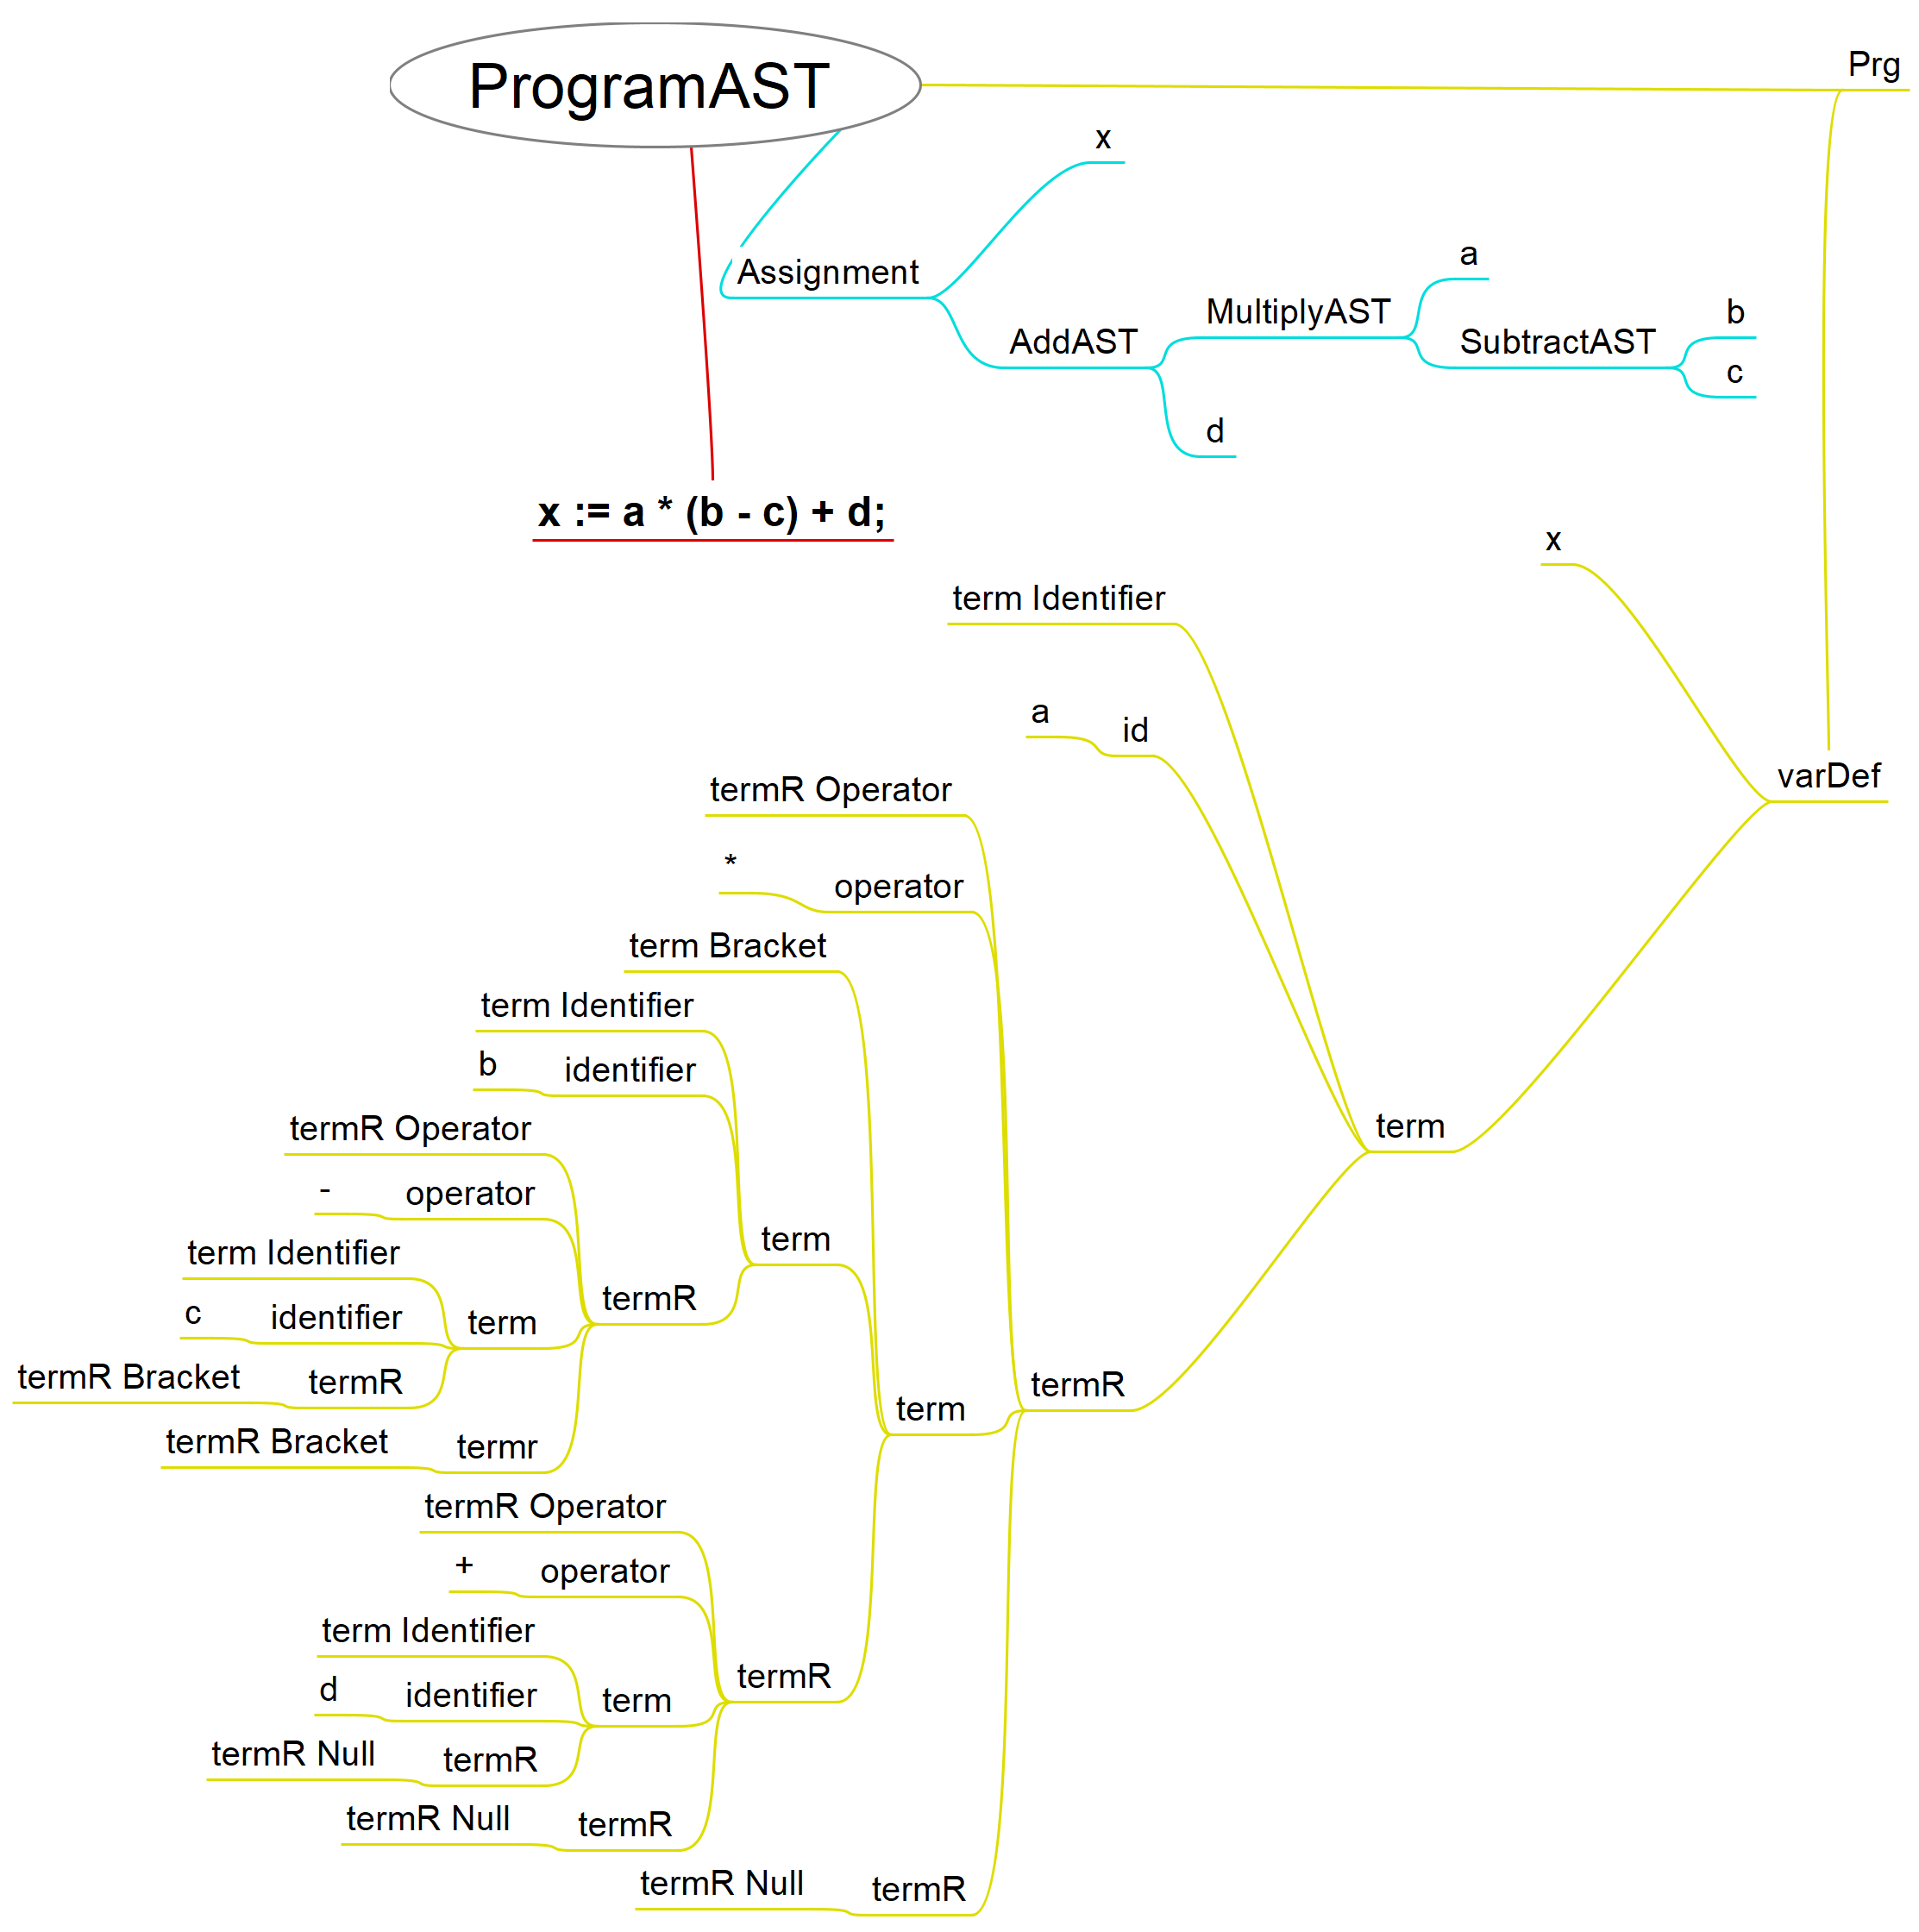
\includegraphics[width=1.0\linewidth]{images/parser-to-ast}
	\caption[Parser-Baum und AST]{Parser-Baum und AST anhand eines kleinen Beispiels}
	\label{fig:parseast}
\end{figure}

\subsection{Lexer}

Der Lexer wandelt den übergebenen Programmcode mithilfe von Regular Expressions in Tokens um. Diese enthalten jeweils den zugehörigen Text, den Typ und die Position im Text, welche später beispielsweise zum Anzeigen von Exceptions benötigt wird. 

\subsection{Parser-Baum}\label{subsection:parser}



Beim Parser-Baum handelt es sich um eine direkte Umsetzung aus der gegebenen Sprachsyntax. 
\begin{figure}[tbh]
	%\centering
	\hspace{-0.1\linewidth}
	%\fbox{}
	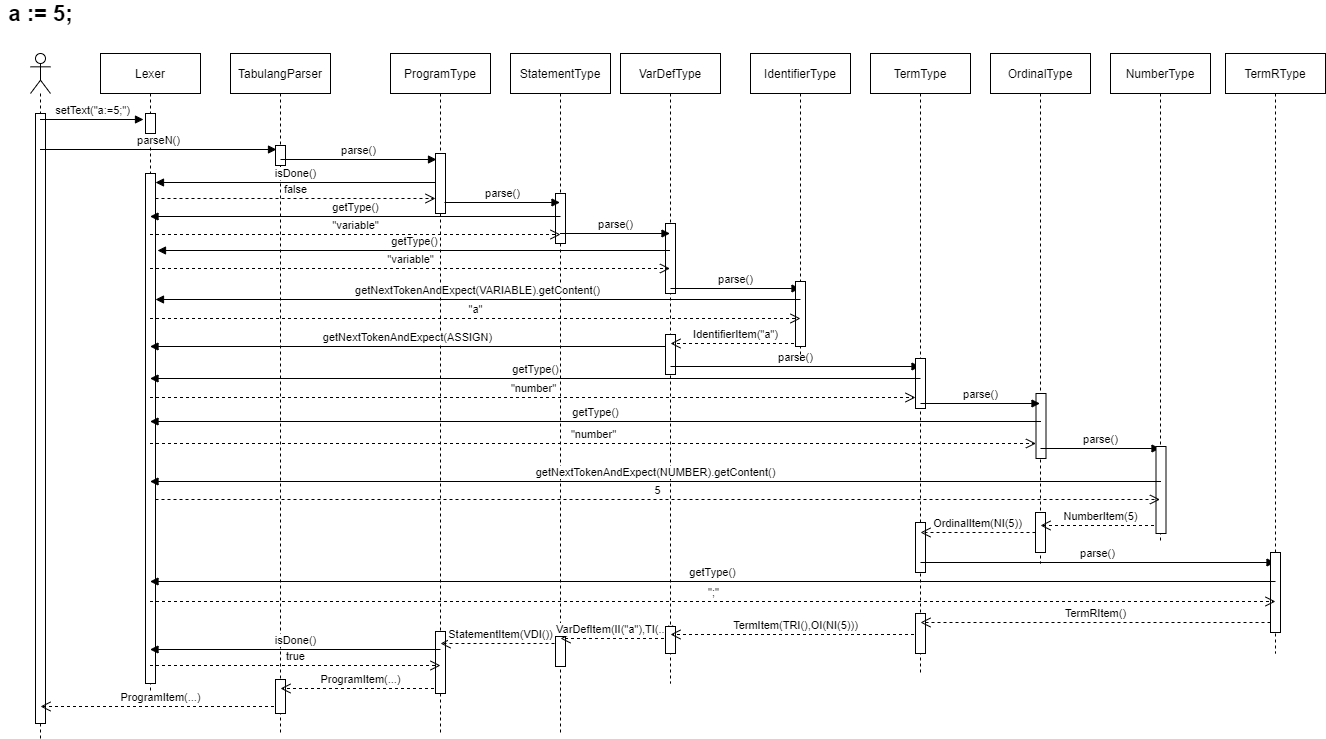
\includegraphics[width=1.2\linewidth]{images/sequenzdiagramm}
	\caption[Sequenzdiagramm Parser]{Sequenzdiagramm für die Erstellung des Parser-Baums}
	\label{fig:sequenzdiagramm}
\end{figure}


\subsection{Abstract-Syntax-Tree (AST)}\label{subsection:ast}

